%% LyX 1.5.3 created this file.  For more info, see http://www.lyx.org/.
%% Do not edit unless you really know what you are doing.
\documentclass[english]{article}
\usepackage[T1]{fontenc}
\usepackage[latin9]{inputenc}
\setlength{\parskip}{\medskipamount}
\setlength{\parindent}{0pt}
\usepackage{url}
\usepackage{amsmath}
\usepackage{graphicx}
\usepackage{amssymb}
\usepackage{graphicx}

\makeatletter
%%%%%%%%%%%%%%%%%%%%%%%%%%%%%% Textclass specific LaTeX commands.
\usepackage{Sweave}
\newcommand{\Rcode}[1]{{\texttt{#1}}}
\newcommand{\Robject}[1]{{\texttt{#1}}}
\newcommand{\Rcommand}[1]{{\texttt{#1}}}
\newcommand{\Rfunction}[1]{{\texttt{#1}}}
\newcommand{\Rfunarg}[1]{{\textit{#1}}}
\newcommand{\Rpackage}[1]{{\textit{#1}}}
\newcommand{\Rmethod}[1]{{\textit{#1}}}
\newcommand{\Rclass}[1]{{\textit{#1}}}

%%%%%%%%%%%%%%%%%%%%%%%%%%%%%% User specified LaTeX commands.
% Meta information - fill between {} and do not remove %
% \VignetteIndexEntry{Factor Analysis in R}
% \VignetteDepends{}
% \VignetteKeywords{models, multivariate}
% \VignettePackage{FAiR}
\usepackage{fullpage}
\usepackage{times}

\usepackage{babel}
\makeatother

\begin{document}

\title{Pop-Up Menus in FA$i$R}


\author{Ben Goodrich}

\maketitle
\textbf{This vignette is intended to be a quick reference that defines
terms and illustrates how to use the pop-up menus. Large parts will
not make a great deal of sense outside the introduction to SEFA and
lexical optimization in Goodrich (2008a) and its (unwritten) extension
to EFA in Goodrich (2008b).}

\tableofcontents{}

\newpage{}


\section{Notation}

Some notation is provided so that the reader can refer back to it.
For simplicity, I do not distinguish the notation for a population
parameter from the notation for an estimate of that population parameter
here.

\begin{itemize}
\item $n$ is the number of outcome variables
\item $\mathbf{S}$ is the $n\times n$ correlation matrix among outcomes
in the sample
\item $r_{1}\geq1$ is the number of factors (at the first level)
\item $\boldsymbol{\beta}$ is the $n\times r_{1}$ primary pattern matrix
(at the first level)
\item $\boldsymbol{\Phi}$ is the $r_{1}\times r_{1}$ correlation matrix
among primary factors (at the first level)
\item $\boldsymbol{\Theta}^{2}$ is the $n\times n$ diagonal covariance
matrix among unique factors (at the first level)
\item $\mathbb{E}\left[\mathbf{S}\right]=\mathbf{C}=\boldsymbol{\beta\Phi\beta}^{\prime}+\boldsymbol{\Theta}^{2}$
is the $n\times n$ expectation of $\mathbf{S}$ as a function of
parameters (at the first level)
\item $\boldsymbol{\Pi}=\boldsymbol{\beta\boldsymbol{\Phi}}$ is the $n\times r_{1}$
primary structure matrix (at the first level)
\item $\boldsymbol{\Gamma}=\boldsymbol{\beta}\times\boldsymbol{\Pi}$ is
the $n\times r_{1}$ factor contribution matrix (at the first level)
where $\times$ indicates element-by-element multiplication rather
than matrix multiplication 
\item $\mathbf{D}^{-2}=\textrm{Diag}\left(\boldsymbol{\Phi}^{-1}\right)$
is the $r_{1}\times r_{1}$ diagonal of the inverse of the correlation
matrix among primary factors (at the first level)
\item $\mathbf{D}=\left[\mathbf{D}^{-2}\right]^{-\frac{1}{2}}$ is the $r_{1}\times r_{1}$
correlation matrix between primary and reference factors (at the first
level)
\item $\boldsymbol{\Psi}=\mathbf{D}\boldsymbol{\Phi}^{-1}\mathbf{D}$ is
the $r_{1}\times r_{1}$ correlation matrix among reference factors
(at the first level)
\item $\boldsymbol{\Upsilon}=\boldsymbol{\beta}\mathbf{D}$ is the $n\times r_{1}$
reference structure matrix (at the first level)
\item $r_{2}\geq0$ is the number of second-order factors
\item $\boldsymbol{\Delta}$ is the $r_{1}\times r_{2}$ second-order primary
pattern matrix
\item $\boldsymbol{\Xi}$ is the $r_{2}\times r_{2}$ correlation matrix
among second-order primary factors
\item $\boldsymbol{\Omega}^{2}$ is the $r_{1}\times r_{1}$ diagonal covariance
matrix among second-order unique factors
\item $\boldsymbol{\Phi}=\boldsymbol{\Delta\Xi\Delta}^{\prime}+\boldsymbol{\Omega}^{2}$
is the $r_{1}\times r_{1}$ second-order equation for the primary
factors as a function of second-order parameters
\item $\boldsymbol{\digamma}=\boldsymbol{\Delta}\boldsymbol{\Xi}$ is the
$r_{2}\times r_{1}$ primary structure matrix at the second level
\item $\boldsymbol{\Game}=\boldsymbol{\Delta}\times\boldsymbol{\digamma}$
is the $r_{2}\times r_{1}$ factor contribution matrix at the second
level where $\times$ indicates element-by-element multiplication
rather than matrix multiplication
\item $\mathbf{Z}^{-2}=\textrm{Diag}\left(\boldsymbol{\Xi}^{-1}\right)$
is the $r_{2}\times r_{2}$ diagonal of the inverse of the correlation
matrix among primary factors at the second level
\item $\mathbf{Z}=\left[\mathbf{Z}^{-2}\right]^{-\frac{1}{2}}$ is the $r_{2}\times r_{2}$
correlation matrix between primary and reference factors at the second
level
\item $\boldsymbol{\mho}=\boldsymbol{\Delta}\mathbf{Z}$ is the $r_{1}\times r_{2}$
reference structure matrix at the second level
\end{itemize}

\section{SEFA or CFA via \texttt{Factanal()}}

To start this sequence, I typed the command \\ \Rcode{mental.tests <- Factanal(covmat = Harman74.cor, factors = 5, model = "SEFA")}


\subsection{Simultaneous Second-Order Model}

If $r_{1}\geq3$, the user will be asked whether to estimate a simultaneous
second-order model, which decomposes the correlation matrix among
first-order primary factors as a function of fewer second-order factors.
For example, some people define ``general intelligence'' to be the
second-order factor that drives various first-order (primary) mental
abilities. If a second-order model is estimated, and if $r_{1}\geq5$,
the user will be asked how many second-order factors $\left(r_{2}\right)$
to extract. 

If a second-order model is specified, the tasks are to set bounds
on the correlations among second-order factors (if $r_{2}\geq2$),
to fix values of the second-order coefficients (for CFA and mixed
SEFA models), to set bounds on the second-order coefficients, and
to choose a mapping rule for the second-order coefficients (if $r_{2}\geq2$
in a SEFA model).


\subsubsection{Deciding on a Simultaneous Second-Order Model\label{sub:2nd}}

%
\begin{figure}
\caption{Simultaneous Second-Order Model with $r_{2}=2$}
\label{fig:simultaneous}

\noindent \begin{centering}
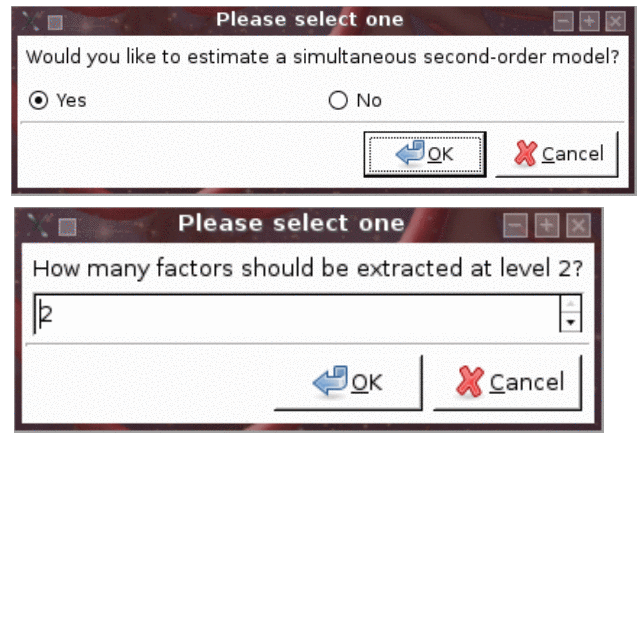
\includegraphics{screenshots/simultaneous/simultaneous}
\par\end{centering}
\end{figure}
Figure \ref{fig:simultaneous} shows two dialog boxes. First, the
user is asked whether to estimate a simultaneous second-order model.
If the user were to choose ``No'' at this point, there would be no
second-order model and the user would then be asked about bounds on
the off-diagonals of $\boldsymbol{\Phi}$. Such a dialog would be
similar to that in section \ref{sub:2nd_bounds_cor}, except that
``level 2'' would be replaced by ``level 1''. Then the dialog would
cut directly to that described in section \ref{sub:1st}.

For the sake of completeness, I will assume that the user answered
``Yes'' to the question of whether a simultaneous second-order model
should be estimated. At this point, the dialog asks the user to specify
the value of $r_{2}$. If $r_{1}=3$ or $r_{1}=4$, then $r_{2}$
can only be one. If $r_{1}\geq5$, then $r_{2}$ can be two. If $r_{1}\geq6$,
then $r_{2}$ can be three. Rarely would one need to estimate a model
with larger numbers for $r_{1}$ and $r_{2}$. I will assume that
the user has chosen $r_{2}=2$.


\subsubsection{Bounds on the Correlations Among the Primary Factors $\left(\boldsymbol{\Xi}\right)$
at Level 2\label{sub:2nd_bounds_cor}}

%
\begin{figure}
\caption{Slightly Limiting the Bounds on the Correlation Between Second-Order
Primary Factors}
\label{fig:bounds_Xi}

\noindent \begin{centering}
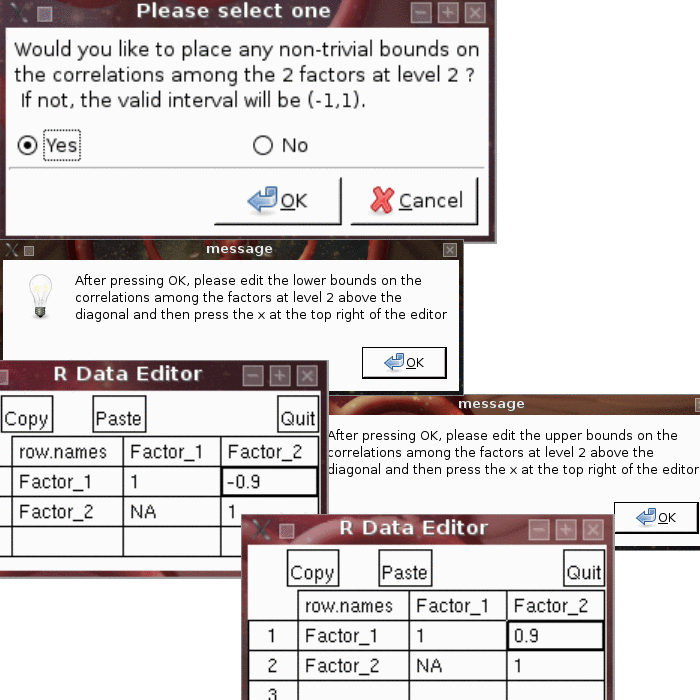
\includegraphics{screenshots/simultaneous/bounds}
\par\end{centering}


\end{figure}
The next menu asks about bounds on the off-diagonals of $\boldsymbol{\Xi}$,
as shown in figure \ref{fig:bounds_Xi}. If $r_{2}\leq1$, this question
would not be asked.

Since $\boldsymbol{\Xi}$ is constrained to be a positive definite
correlation matrix, the off-diagonals cannot exceed $\pm1$. It is
possible, but often not necessary, to impose stricter bounds. Occasionally,
there can be optimization difficulties if any correlation gets too
close to $\pm1$, and in that case the user may want to narrow the
acceptable interval to $\left(-0.9,0.9\right)$ or so.

If ``No'' is chosen, the dialog will skip to section \ref{sub:peg2}
using the $\left(-1,1\right)$ interval for all correlations among
second-order factors. For the sake of completeness, I will assume
the user answers ``Yes'' to this question.

Since $\boldsymbol{\Xi}$ is a correlation matrix, the diagonal elements
are constrained to be $1.0$ and the diagonal elements will be ignored
if they are changed. Since a correlation matrix is symmetric, it is
not necessary to change the values below the diagonal and they will
be ignored regardless. It is only necessary to specify the values
above the diagonal. In this case, I have specified a lower bound of
$-0.9$ on the only correlation among the two primary factors at level
2, which is a very conservative choice. 

When satisfied with the lower-bounds on the off-diagonals of $\boldsymbol{\Xi}$,
click the $\mathbf{x}$ at the top right (or {}``Quit'', but {}``Quit''
does not appear in the Windows version). Once $\mathbf{x}$ is pressed,
the process is repeated for the upper bounds on the off-diagonals
of $\boldsymbol{\Xi}$.


\subsubsection{Specifying Values of the Primary Pattern Matrix $\left(\boldsymbol{\Delta}\right)$
at Level 2\label{sub:peg2}}

%
\begin{figure}
\caption{(Not) Pegging Coefficients to Specified Values}
\label{fig:peg2}

\noindent \begin{centering}
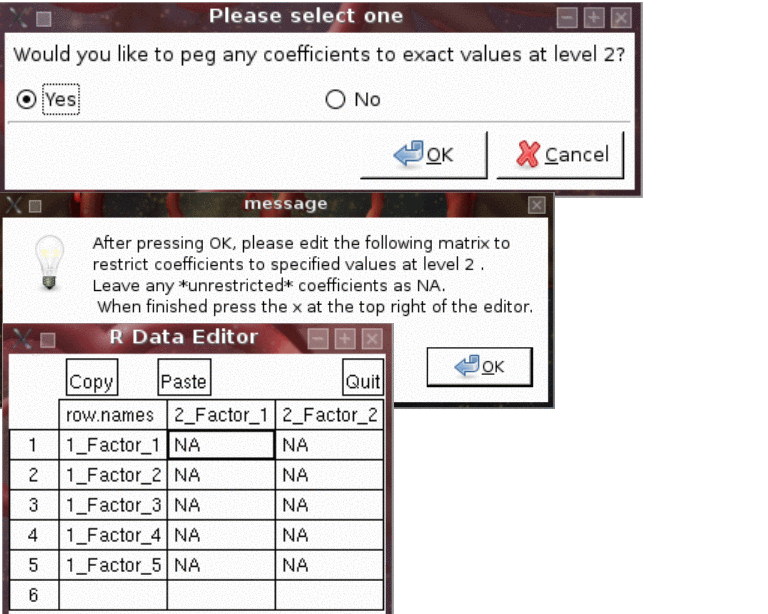
\includegraphics{screenshots/simultaneous/fish/fish}
\par\end{centering}


\end{figure}
%
\begin{figure}
\caption{Specifying Informative Bounds on Primary Pattern Coefficients at Level
2}
\label{fig:bounds_Delta}

\noindent \begin{centering}
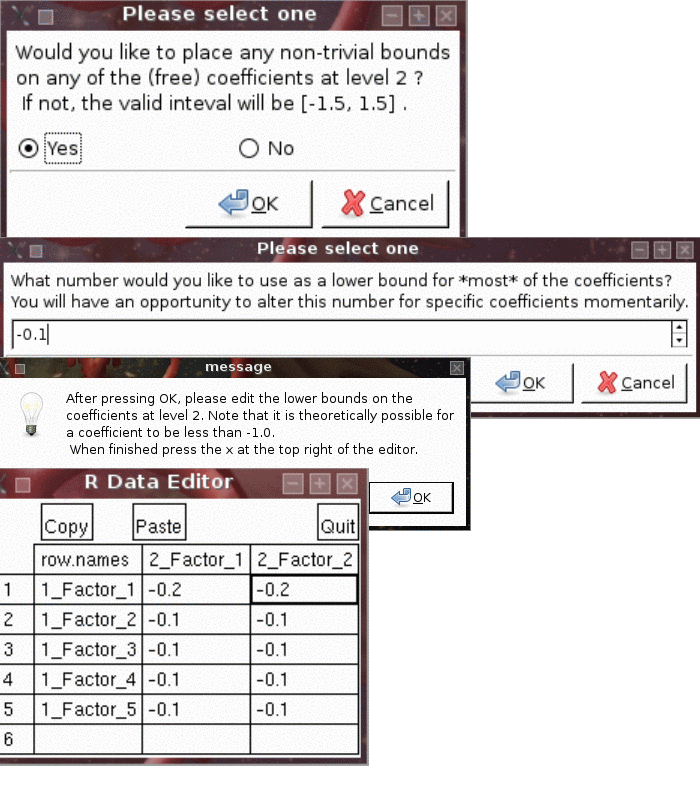
\includegraphics{screenshots/simultaneous/fish/bounds/bounds}
\par\end{centering}
\end{figure}
Since this example is a SEFA, the next dialog (shown in figure \ref{fig:peg2})
asks the user whether any elements of $\boldsymbol{\Delta}$ should
be pegged to specific values. If a CFA model were estimated, this
question would not appear because it is obligatory to peg some elements
of $\boldsymbol{\Delta}$ in a CFA model. In a SEFA model, it is possible
to answer ``No'' to this question in order to estimate a {}``pure''
SEFA model. However, for illustrative purposes, I will assume that
the user answers ``Yes'' to estimate a ``mixed SEFA'' model.

At this point, the user should change the appropriate cells of $\boldsymbol{\Delta}$
from NA to numbers. For example, the user might change the first row
to $\begin{bmatrix}1.0 & 0.0\end{bmatrix}$ to make the first factor
at the second level collinear with the first factor at the first level.
Any elements of $\boldsymbol{\Delta}$ that are to be \emph{unrestricted}
should be left as NA.

If a CFA model were being estimated, it would be necessary to specify
restrictions on $\boldsymbol{\Delta}$ to satisfy the theorem on rotational
indeterminancy in Howe (1955). Namely there should be at least $r_{2}-1$
zeros in each column of $\boldsymbol{\Delta}$ such that all $r_{2}$
submatrices of $\boldsymbol{\Delta}$ with zeros in the $p$th column
of $\boldsymbol{\Delta}$ are of rank $r_{2}-1$.

In this case, a mixed SEFA model is being estimated, so it is possible
to specify fewer cells of $\boldsymbol{\Delta}$ including no restricted
cells at all. Here I assume the user has changed his or her mind about
restrictions on $\boldsymbol{\Delta}$ and now wants all cells to
be unrestricted. Thus, all cells remain NA.


\subsubsection{Bounds on Cells of the Primary Pattern Matrix $\left(\boldsymbol{\Delta}\right)$
at Level 2\label{sub:2nd_bounds_fish}}

The next question is what bounds should be placed on the cells of
$\boldsymbol{\Delta}$. The dialog shown in figure \ref{fig:bounds_Delta}
is similar to that in section \ref{sub:2nd_bounds_cor}, except that
the bounds are being placed on the cells of $\boldsymbol{\Delta}$
rather than the off-diagonals of $\boldsymbol{\Xi}$. It is always
possible to select ``No'', but doing so does not make the cells of
$\boldsymbol{\Delta}$ unbounded. Rather, fairly wide bounds are used,
in particular $\pm1.5$. In some cases, it may be necessary to specify
wider bounds, but in most cases if the user answers ``Yes'', it would
be to narrow the bounds.

If the user specifies bounds, the number chosen in the next dialog
fills every free cell of the subsequent editable menu. The fixed coefficients,
if any, would be filled with their values. The user can then edit
particular cells as necessary. Here I have changed both cells in the
first row to $-0.2$ to permit a more diffuse positive manifold for
the first second-order factor.

It should be emphasized that it is possible for coefficients to be
less than $-1.0$ when $r_{2}>1$. The decision here to limit the
cells of $\boldsymbol{\Delta}$ to be greater than $-0.2$ or $-0.1$
is a \emph{substantive} constraint that can be wrong and can be tested.
If strong bounds are used, it may be best to specify \Rcode{boundary.enforcement = 2}
in the call to \Rcode{Factanal}.

When finished, press $\mathbf{x}$ (or {}``Quit'' but {}``Quit''
does not appear on the Windows version), to repeat this procedure
for the upper bounds on the cells of $\boldsymbol{\Delta}$. It is
necessary that some of the valid intervals for the cells of $\boldsymbol{\Delta}$
include zero so that the Howe (1955) theorem can be satisfied in a
SEFA model. It is difficult to generally prove when inequality restrictions
on coefficients are sufficient to eliminate rotational indeterminacy,
so the Howe (1955) theorem is recommended.


\subsubsection{Mapping Rules for the Primary Pattern Matrix $\left(\boldsymbol{\Delta}\right)$
at Level 2}

%
\begin{figure}
\caption{Mapping Rules at Level 2 in a SEFA}
\label{fig:map2}

\noindent \begin{centering}
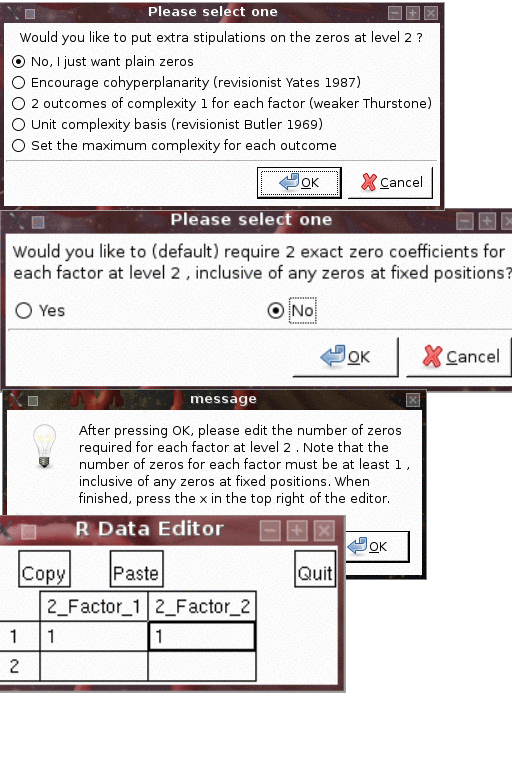
\includegraphics{screenshots/simultaneous/fish/SEFA/SEFA}
\par\end{centering}
\end{figure}
In the SEFA model presumed here, the questions shown in figure \ref{fig:map2}
are very important and pertain to the mapping rule used to squash
certain cells of $\boldsymbol{\Delta}$ to zero. If a CFA model were
being estimated, this question would not appear because the Howe (1955)
theorem must be satisfied by \emph{a priori} restrictions. Let $b_{p}$
be the number of zeros required for the $p$th column of $\boldsymbol{\Delta}$.
Most of the mapping rules at the second level are defined on the reference
structure matrix $\left(\check{\boldsymbol{\mho}}\right)$ and the
factor contribution matrix $\left(\check{\boldsymbol{\Game}}\right)$,
rather than the primary pattern matrix ($\check{\boldsymbol{\Delta}}$),
where the supra-check indicates a prelimary matrix that is constructed
by filling the free elments with $\boldsymbol{\theta}$ (in symbols)
or \Rcode{par} (in R syntax). By ``smallest'', I always mean in absolute
value. The distinctions between mapping rules are fairly minor in
this case when $r_{2}=2$, but are defined in general as follows:

\begin{itemize}
\item ``No, I just want plain zeros''. This mapping rule simply squashes
the $b_{p}$ smallest elements in the $p$th column of $\check{\boldsymbol{\mho}}$
to zero, implying that $\boldsymbol{\Delta}_{p}$ has $b_{p}$ zeros.
\item ``Encourage cohyperplanrity (revisionist Yates 1987)''. This mapping
rule squashes $r_{2}-1$ elements in the $p$th column of $\boldsymbol{\Delta}$
using the following piecewise function $\forall q\neq p$:\begin{eqnarray*}
\Delta_{jp} & = & \begin{cases}
0 & \textrm{if}\,\,\check{\Game}_{jq}-\check{\Game}_{jq}=\max\left\{ \check{\boldsymbol{\Game}}_{q}-\check{\boldsymbol{\Game}}_{p}\right\} \\
\check{\Delta}_{jp} & \textrm{otherwise,}\end{cases}\end{eqnarray*}
which tends to place a zero in the $p$th column of $\boldsymbol{\Delta}$
at the row where the factor contribution of some other column is large
for each of the remaining columns.
\item ``$r_{2}$ `outcomes' (really primary factors) of complexity $r_{2}-1$
for each factor (weaker Thurstone)''. This mapping rule is similar
to the ``plain zeros'' mapping rule in that $r_{2}$ small elements
in the $p$th column of $\check{\boldsymbol{\mho}}$ are squashed
to zero, except that there is an additional stipulation that no ``outcome''
(really primary factor) is of complexity less than $r_{2}-1$ where
the complexity of the $j$th ``outcome'' (primary factor) is the number
of non-zeros in $\boldsymbol{\mho}_{j}$. However, any ``non-zero''
coefficient can be arbitrarily close to zero. Thus, each column of
$\boldsymbol{\Delta}$ will have $r_{2}$ \emph{exact} zeros.
\item ``Unit complexity basis (revisionist Butler 1969)''. This mapping
rule uses the dishinguishability weights defined in Yates (1987) to
select $r_{2}$ primary factors that are of unit complexity. In particular,
let\begin{eqnarray*}
\check{w}_{p} & = & \frac{1}{\sum\check{\Game}_{\centerdot\centerdot}}\sum_{j=1}^{r_{1}}\check{\Game}_{jp}\end{eqnarray*}
where $\sum\check{\Game}_{\centerdot\centerdot}=\sum_{j=1}^{r_{1}}\sum_{p=1}^{r_{2}}\check{\Game}_{jp}$
is the weight applied the the $p$th second-order factor such that
$\sum_{p=1}^{r_{2}}w_{p}=1$. This equation is similar to equation
$118$ in Yates (1987, p.~145). Then let\begin{eqnarray*}
\check{c}_{j} & = & \frac{\sum_{p=1}^{r_{2}}\check{w}_{p}\check{\Delta}_{jp}}{\sum_{p=1}^{r_{2}}\check{\Game}_{jp}}\end{eqnarray*}
be the directional cosine between $\check{\boldsymbol{\Delta}}_{j}$
and the (weighted) centroid of $\check{\boldsymbol{\Delta}}$, which
is the same as equation $119$ in Yates (1987, p.~145). Finally,
let \begin{eqnarray*}
d_{j}^{w} & = & \min\left\{ 1,\frac{\left(r_{2}\right)^{2}}{r_{2}-1}\check{c}_{j}\left(\check{c}_{j}-1\right)\right\} \end{eqnarray*}
be the distinguishability weight for $\check{\boldsymbol{\Delta}}_{j}$,
which is the same as equation $78a$ in Yates (1987, p.~112). Then,
$\forall p$ choose a first-order factor to be of unit complexity
among first-order factors where $\check{\Game}_{jp}=\max\left\{ \boldsymbol{\check{\Game}}_{j}\right\} $
such that $d_{j}^{w}$ is maximal. For such first-order factors, squash
$\boldsymbol{\Delta}_{j}$ to zero $\forall q\neq p$. At the end
of these steps, there will be $r_{2}$ first-order factors that are
collinear with the second-order primary axes and there will be $r_{2}-1$
zeros in each column of $\boldsymbol{\Delta}$.
\item {}``Set the maximum complexity for each outcome.'' This mapping
rule is similar to the ``plain zeros'' mapping rule, except that it
is applied to each \emph{row} of $\boldsymbol{\Delta}$ rather than
the columns. In general, $\forall j$, the user can choose a number
between $1$ and $r_{2}$ for the maximum number of non-zero coefficients
in $\boldsymbol{\Delta}_{j}$. More details on this mapping rule are
given in section X.
\end{itemize}
In some cases, $b_{p}$ may be greater than the number of zeros created
by whichever mapping rule is chosen. In that case, the remaining zeros
are filled in by squashing the $b_{p}$ smallest elements in the $p$th
column of the \emph{recalculated} reference structure matrix after
the mapping rule has been applied and some reference structure correlations
are zero. Thus, it is necessary to specify $b_{p}$, and the dialog
box for doing so is also shown in figure \ref{fig:map2}. By default,
the user is asked whether to set $b_{p}=r_{2}\,\forall p$, which
can be accepted by answering ``Yes'' to the following question but
here I answer ``No'' to specify\textbf{ }$b_{p}=r_{2}-1\,\forall p$.

This concludes the dialog boxes for the second-order model.


\subsection{First-Order Model\label{sub:1st}}

The tasks are to set bounds on the correlations among first-order
factors (if a second-order model is not estimated), to fix values
of the first-order coefficients (for CFA and mixed SEFA models), to
set bounds on the first-order coefficients, and to choose a mapping
rule for the first-order coefficients (if $r_{2}\geq2$ in a SEFA
model).

Note that if there is no second-order model, the user will be asked
about bounds on the off-diagonals of $\boldsymbol{\Phi}$. This dialog
is similar to that in section \ref{sub:2nd_bounds_cor}, except that
``level 2'' is replaced by ``level 1'' in the prompts.


\subsubsection{Specifying Values of the Primary Pattern Matrix $\left(\boldsymbol{\beta}\right)$
at Level 1}

%
\begin{figure}
\caption{(Not) Specifying Values for the Primary Pattern Coefficients at Level
1}
\label{fig:pegs1}

\noindent \begin{centering}
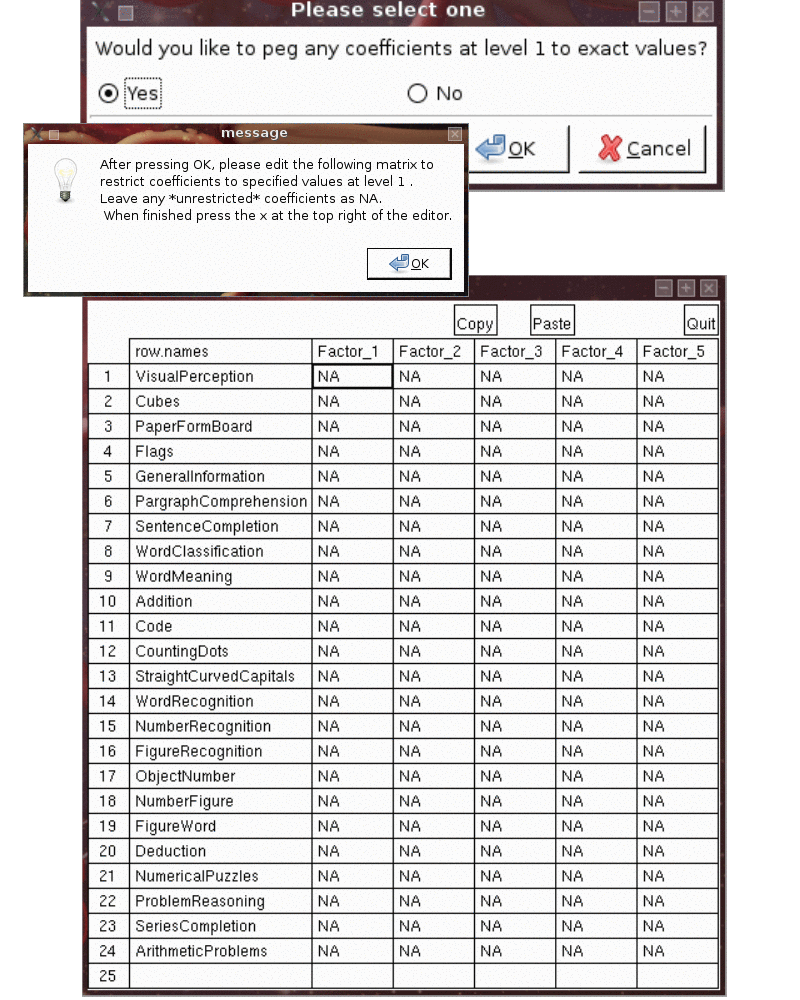
\includegraphics{screenshots/firstorder/pegs/pegs}
\par\end{centering}


\end{figure}
Since this example is a SEFA, the dialog shown in figure \ref{fig:pegs1}
asks the user whether any elements of $\boldsymbol{\beta}$ should
be pegged to specific values. If a CFA model were estimated, this
question would not appear because it is obligatory to peg some elements
of $\boldsymbol{\beta}$ in a CFA model. In a SEFA model, it is possible
to answer ``No'' to this question to estimate a {}``pure'' SEFA
model. However, for illustrative purposes, I will assume that the
user answers ``Yes'' to estimate a {}``mixed'' SEFA model.

At this point, the user should change the appropriate cells of $\boldsymbol{\beta}$
from NA to numbers. For example, the user might change the first row
to $\begin{bmatrix}\textrm{NA} & 0.0 & 0.0 & 0.0 & 0.0\end{bmatrix}$
to make the first factor collinear with visual perceptiveness. Any
elements of $\boldsymbol{\beta}$ that are \emph{unrestricted} should
be left as NA. Continuing this example, by leaving the first factor
unrestricted for the visual perception test, the user allows the test
to have measurement error. 

If a CFA model were being estimated, it would be necessary to specify
restrictions on $\boldsymbol{\beta}$ to satisfy the theorem on rotational
indeterminancy in Howe (1955). Namely there should be at least $r_{1}-1$
zeros in each column of $\boldsymbol{\beta}$ such that all $r_{1}$
submatrices of $\boldsymbol{\beta}$ with zeros in the $p$th column
of $\boldsymbol{\beta}$ are of rank $r_{1}-1$.

In this case, a SEFA model is being estimated, so it is possible to
specify fewer cells of $\boldsymbol{\beta}$ including no restricted
cells at all. Here I assume the user has changed his or her mind about
restrictions on $\boldsymbol{\beta}$ and now wants all cells to be
unrestricted. Thus, all cells are left as NA.


\subsubsection{Bounds on Cells of the Primary Pattern Matrix $\left(\boldsymbol{\beta}\right)$
at Level 1}

%
\begin{figure}
\caption{Specifying Bounds on the Primary Pattern Coefficients at Level 1}
\label{fig:bounds1}

\noindent \begin{centering}
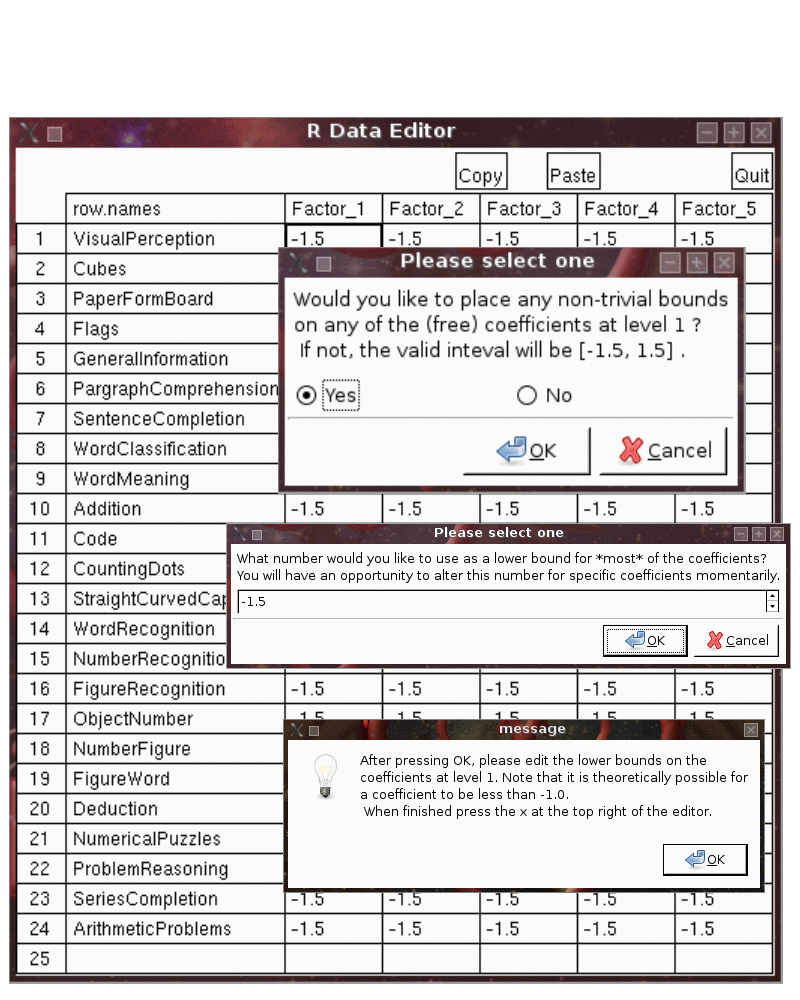
\includegraphics{screenshots/firstorder/bounds/bounds}
\par\end{centering}
\end{figure}
The next question is what bounds should be placed on the cells of
$\boldsymbol{\beta}$. The dialog in figure is similar to that in
section \ref{sub:2nd_bounds_fish}, except that the bounds are being
placed on the cells of the primary pattern matrix at level 1 $\left(\boldsymbol{\beta}\right)$
rather than the primary pattern matrix at level 2 $\left(\boldsymbol{\Delta}\right)$.
It should be kept in mind that the model is estimated on a \emph{correlation}
matrix of outcomes $\left(\mathbf{S}\right)$ when choosing bounds.
Thus, it is somewhat uncommon --- but nevertheless possible --- for
a coefficient to be greater than $\pm1$. It is always possible to
select ``No'', but doing so does not make the cells of $\boldsymbol{\beta}$
unbounded. Rather, fairly wide bounds are used, in particular $\pm1.5$.
In some cases, it may be necessary to specify wider bounds, but in
most cases if the user answers ``Yes'', it would be to narrow the
bounds.

After an initial number is chosen to fill all the cells in the editor,
the user can change some or all of the cells as necessary. For example,
to estimate the model under a positive manifold restriction, the user
could set all lower bounds to $-0.2$ or something. When finished
with the lower bounds, click the $\mathbf{x}$, at which point the
process is repeated for the upper bounds. It is important for some,
if not all, of the valid intervals to include zero in a SEFA model
so that the rotational indeterminancy can be eliminated by mapping
some coefficients to zero.


\subsubsection{Mapping Rules for Coefficients at Level 1\label{sub:maps}}

%
\begin{figure}
\caption{Mapping Rules at Level 1 in a SEFA Model}
\label{fig:maps1}

\noindent \begin{centering}
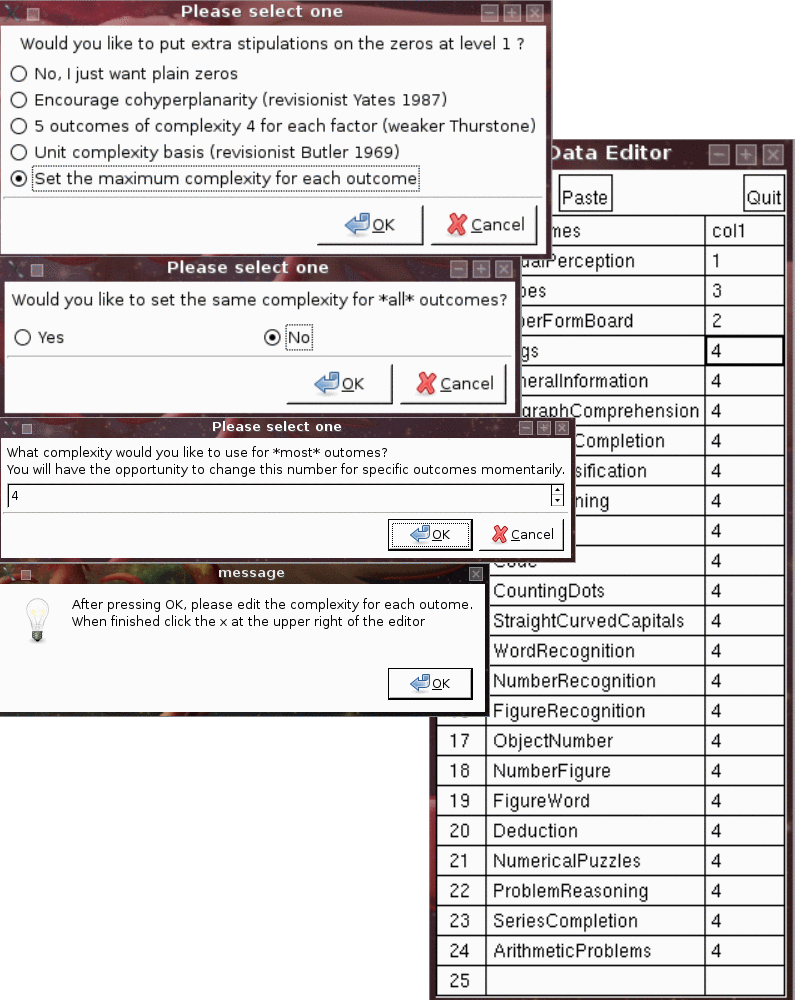
\includegraphics{screenshots/firstorder/SEFA/SEFA}
\par\end{centering}


\end{figure}
In the SEFA model presumed here, the next question is very important
and pertains to the mapping rule used to squash certain cells of $\boldsymbol{\beta}$
to zero. If a CFA model were being estimated, this questions in figure
\ref{fig:maps1} would not appear because the Howe (1955) theorem
would be satisfied by \emph{a priori} restrictions.

Let $b_{p}$ be the number of zeros required for the $p$th column
of $\boldsymbol{\beta}$. Most of the mapping rules at the second
level are defined on the reference structure matrix $\left(\check{\boldsymbol{\Upsilon}}\right)$
and the factor contribution matrix $\left(\check{\boldsymbol{\Gamma}}\right)$,
rather than the primary pattern matrix ($\check{\boldsymbol{\beta}}$),
where the $\check{}$ indicates a prelimary matrix that is constructed
by filling the free elments with $\boldsymbol{\theta}$ (in symbols)
or \Rcode{par} (in R syntax). By ``smallest'', I always mean in absolute
value. The mapping rules in the first dialog box in figure \ref{fig:maps1}
are defined as follows:

\begin{itemize}
\item ``No, I just want plain zeros''. This mapping rule simply squashes
the $b_{p}$ smallest elements in the $p$th column of $\check{\boldsymbol{\Upsilon}}$
to zero, implying that $\boldsymbol{\beta}_{p}$ has $b_{p}$ zeros.
\item ``Encourage cohyperplanrity (revisionist Yates 1987)''. This mapping
rule squashes $r_{2}-1$ elements in the $p$th column of $\boldsymbol{\beta}$
using the following piecewise function $\forall q\neq p$:\begin{eqnarray*}
\beta_{jp} & = & \begin{cases}
0 & \textrm{if}\,\check{\Gamma}_{jq}-\check{\Gamma}_{jq}=\max\left\{ \check{\boldsymbol{\Gamma}}_{q}-\check{\boldsymbol{\Gamma}}_{p}\right\} \\
\check{\beta}_{jp} & \textrm{otherwise,}\end{cases}\end{eqnarray*}
which tends to place the zeros for the $p$th column of $\boldsymbol{\beta}$
in the rows where the factor contribution of some other column is
large.
\item ``$r_{1}$ outcomes of complexity $r_{1}-1$ for each factor (weaker
Thurstone)''. This mapping rule is similar to the ``plain zeros''
mapping rule in that $r_{1}$ small elements in the $p$th column
of $\check{\boldsymbol{\Upsilon}}$ are squashed to zero, except that
there is an additional stipulation that no outcome is of complexity
less than $r_{1}-1$ where the complexity of the $j$th outcome is
the number of non-zeros in $\boldsymbol{\Upsilon}_{j}$. However,
any ``non-zero'' coefficient can be arbitrarily close to zero. Thus,
each column of $\boldsymbol{\beta}$ will have $r_{1}$ \emph{exact}
zeros.
\item ``Unit complexity basis (revisionist Butler 1969)''. This mapping
rule uses the dishinguishability weights defined in Yates (1987) to
select $r_{1}$ outcomes to be of unit complexity. In particular,
let\begin{eqnarray*}
\check{w}_{p} & = & \frac{1}{\sum\Gamma_{\centerdot\centerdot}}\sum_{j=1}^{n}\check{\Gamma}_{jp}\end{eqnarray*}
where $\sum\Gamma_{\centerdot\centerdot}=\sum_{j=1}^{n}\sum_{p=1}^{r_{1}}\check{\Gamma}_{jp}$
is the weight applied the the $p$th first-order factor such that
$\sum_{p=1}^{r_{1}}w_{p}=1$. This equation is similar to equation
$118$ in Yates (1987, p.~145). Then let\begin{eqnarray*}
\check{c}_{j} & = & \frac{\sum_{p=1}^{r_{1}}\check{w}_{p}\check{\beta}_{jp}}{\sum_{p=1}^{r_{1}}\check{\Gamma}_{jp}}\end{eqnarray*}
be the directional cosine between $\check{\boldsymbol{\beta}}_{j}$
and the (weighted) centroid of $\check{\boldsymbol{\beta}}$, which
is the same as equation $119$ in Yates (1987, p.~145). Finally,
let \begin{eqnarray*}
d_{j}^{w} & = & \min\left\{ 1,\frac{\left(r_{1}\right)^{2}}{r_{1}-1}\check{c}_{j}\left(\check{c}_{j}-1\right)\right\} \end{eqnarray*}
be the distinguishability weight for $\check{\boldsymbol{\beta}}_{j}$,
which is the same as equation $78a$ in Yates (1987, p.~112). Then,
$\forall p$ choose a outcome to be of unit complexity among outcomes
where $\check{\Gamma}_{jp}=\max\left\{ \boldsymbol{\check{\Gamma}}_{j}\right\} $
such that $d_{j}^{w}$ is maximal. For such outcomes, squash $\boldsymbol{\beta}_{j}$
to zero $\forall q\neq p$. At the end of these steps, there will
be $r_{1}$ outcomes that are collinear with the first-order primary
axex and there will be $r_{1}-1$ zeros in each column of $\boldsymbol{\beta}$.
\item {}``Set the maximum complexity for each outcome.'' This mapping
rule is similar to the ``plain zeros'' mapping rule, except that it
is applied to each \emph{row} of $\boldsymbol{\beta}$ rather than
the columns. In general, $\forall j$, the user can choose a number
between $1$ and $r_{1}$ for the maximum number of non-zero coefficients
in $\boldsymbol{\beta}_{j}$. This mapping rule is used as an example
in figure \ref{fig:maps1}. It is possible to choose the same complexity
for all rows of $\boldsymbol{\beta}$, in which case a simpler dialog
box is shown. Note that if the complexity of all rows of $\boldsymbol{\beta}$
is $r_{1}-1$, this restriction characterizes Thurstone's (1935) definition
of simple structure, and if the complexity of all rows is $1$, this
restriction implies a perfect cluster configuration. In figure \ref{fig:maps1},
I have chosen to (arbitrarily) specify the complexity of the rows
of $\boldsymbol{\beta}$ on a row-by-row basis, which gives more flexibility
to place restrictions on the model in accordance with prior theory.
\end{itemize}
In some cases, $b_{p}$ may be greater than the number of zeros created
by whichever mapping rule is chosen. In that case, the remaining zeros
are filled in by squashing the $b_{p}$ smallest elements in the $p$th
column of the \emph{recalculated} reference structure matrix after
the mapping rule has been applied and some reference structure correlations
are zero. Thus, it is necessary to specify $b_{p}$. By default, the
user is asked whether to set $b_{p}=r_{1}\,\forall p$, which can
be accepted by answering ``Yes'' to the question in figure \ref{fig:maps1}.


\subsection{Lexical Criteria}

Finally, the user is asked which lexical criteria should be included
in the optimization. Regardless of what options are chosen here, there
will always be criteria that impose necessary constraints on the model
(positive definite correlation matrices, positive specific variances,
etc.) and constraints that the column sums of $\boldsymbol{\Delta}$
(if a second-order model is estimated) and $\boldsymbol{\beta}$ are
positive, which improves the computational efficiency of the algorithm.
Also, regardless of what options are chosen here, the ultimate criterion
will be appended to the end of the criteria that define constraints.
In this case, the model is to be estimated by maximum likelihood,
so the dialog box reminds the user of this. If a second-order model
is not estimated, the choices that mention with ``level 2'' in figure
\ref{fig:lexical} would not appear. 

Pe\~{n}a and Rodriguez (2003) defines a determinant of a correlation
matrix among a set of variables raised to the power of the reciprocal
of the number of variables as the ``effective variance'' of those
variables. The essence of the effective variance is that it can be
meaningfully compared to a different set of variables when the sets
of variables differ in size. The generalized variance is more well-known
statistic and is simply the determinant of the correlation matrix
among a set of variables. The generalized variance can be interpreted
as the hypervolume of a set of unit-length vectors and the effective
variance can be interpreted as {}``the length of the side of the
hypercube whose volume is equal to the determinant (Pe\~{n}a and
Rodriguez 2003, p.~363).'' Both of these concepts are used to define
the criteria / constraints in figure \ref{fig:lexical}:%
\begin{figure}
\caption{Lexical Criteria in SEFA}
\label{fig:lexical}

\noindent \begin{centering}
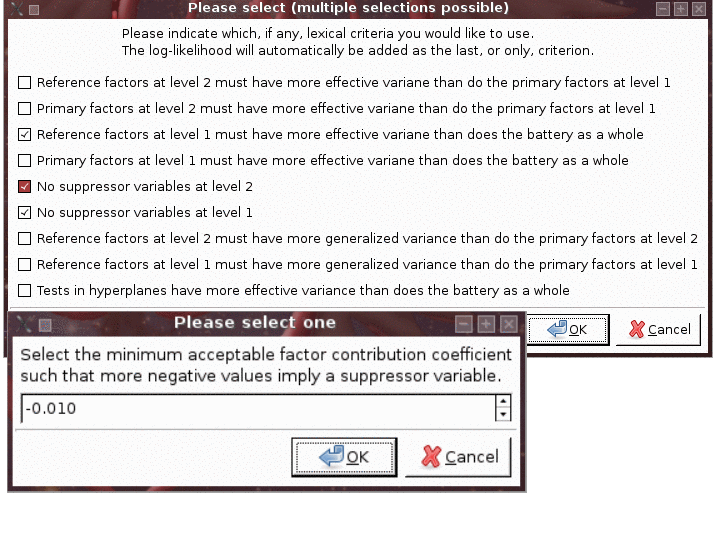
\includegraphics{screenshots/firstorder/constraints/constraints}
\par\end{centering}
\end{figure}


\begin{itemize}
\item {}``Reference factors at level 2 must have more effective variance
than do the primary factors at level 1''. This criterion is formally
defined as \begin{eqnarray*}
 & \begin{cases}
1 & \textrm{if\,}\left|\boldsymbol{\Phi}\right|^{\frac{1}{r_{1}}}\leq\left|\mathbf{Z}\boldsymbol{\Xi}^{-1}\mathbf{Z}\right|^{\frac{1}{r_{2}}}\\
\left|\boldsymbol{\Phi}\right|^{\frac{1}{r_{1}}}-\left|\mathbf{Z}\boldsymbol{\Xi}^{-1}\mathbf{Z}\right|^{\frac{1}{r_{2}}} & \textrm{otherwise,}\end{cases}\end{eqnarray*}
and loosely requires that the reference factors at level 2 be ``less
correlated per variable'' than are the primary factors at level 1.
This criterion tends to push the second-order axes toward the edge
of the configuration of first-order factors.
\item {}``Primary factors at level 2 must have more effective variance
than do the primary factors at level 1''. This criterion is formally
defined as \begin{eqnarray*}
 & \begin{cases}
1 & \textrm{if\,}\left|\boldsymbol{\Phi}\right|^{\frac{1}{r_{1}}}\leq\left|\boldsymbol{\Xi}\right|^{\frac{1}{r_{2}}}\\
\left|\boldsymbol{\Phi}\right|^{\frac{1}{r_{1}}}-\left|\boldsymbol{\Xi}\right|^{\frac{1}{r_{2}}} & \textrm{otherwise,}\end{cases}\end{eqnarray*}
and is similar to the criterion above. In general, it seems that imposing
this restriction on the second-order primary factors is \emph{stronger}
than imposing it on the second-order reference factors and pushes
the second-order axes farther toward the edge of the configuration
of first order factors.
\item {}``Reference factors at level 1 must have more effective variance
than does the battery as a whole''. This criterion is formally defined
as\begin{eqnarray*}
 & \begin{cases}
1 & \textrm{if\,}\left|\boldsymbol{\Psi}\right|^{\frac{1}{r_{1}}}\leq\left|\mathbf{C}\right|^{\frac{1}{n}}\\
\left|\boldsymbol{\Psi}\right|^{\frac{1}{r_{1}}}-\left|\mathbf{C}\right|^{\frac{1}{n}} & \textrm{otherwise,}\end{cases}\end{eqnarray*}
and is similar to the two criteria above except that the comparison
is relative to $\mathbf{C}$. In this case, the criterion loosely
implies that the reference factors at level 1 be {}``less correlated
per variable'' than is the test configuration in common factor space
and encourages the first-order axes to cut through the edges of the
test configuration. 
\item {}``Primary factors at level 1 must have more effective variance
than does the battery as a whole''. This criterion is formally defined
as\begin{eqnarray*}
 & \begin{cases}
1 & \textrm{if\,}\left|\boldsymbol{\Phi}\right|^{\frac{1}{r_{1}}}\leq\left|\mathbf{C}\right|^{\frac{1}{n}}\\
\left|\Phi\right|^{\frac{1}{r_{1}}}-\left|\mathbf{C}\right|^{\frac{1}{n}} & \textrm{otherwise,}\end{cases}\end{eqnarray*}
and is similar to the previous criterion above except that the correlation
among the primary factors at issue. In general, it seems that imposing
this restriction on the primary factors is \emph{stronger} than imposing
it on the reference factors and tends to push the first-order axes
farther out into the edges of the test configuration.
\item ``No suppressor variables at level 2'' Suppressor variables are defined
as variables with negative factor contributions. This criterion is
advocated, albeit somewhat indirectly, in Yates (1987, p.~119) with
respect to level 1, although I can see no reason why it would be any
less applicable to level 2. Prohibiting suppressor variables strikes
me as a reasonable assumption to make in most cases. The criterion
is formally defined as\begin{eqnarray*}
\frac{1}{r_{1}r_{2}}\sum_{j=1}^{r_{1}}\sum_{p=1}^{r_{2}}\mathbb{I}\left\{ \Game_{jp}\geq\underline{\Game}\right\}  & \textrm{where} & \mathbb{I}\left\{ \Game_{jp}\geq\underline{\Game}\right\} =\begin{cases}
1 & \textrm{if\,\,}\Game_{jp}\geq\underline{\Game}\\
0 & \textrm{otherwise,}\end{cases}\end{eqnarray*}
and $\underline{\Game}$ is a threshold for the minimum acceptable
factor contribution that is specified by the user, as shown at the
bottom of figure \ref{fig:lexical}. 
\item ``No suppressor variables at level 1''. This criterion is conceptually
similar to the one above and is formally defined at level 1 as \begin{eqnarray*}
\frac{1}{nr}\sum_{j=1}^{n}\sum_{p=1}^{r}\mathbb{I}\left\{ \Gamma_{jp}\geq\underline{\Gamma}\right\}  & \textrm{where} & \mathbb{I}\left\{ \Gamma_{pj}\geq\underline{\Gamma}\right\} =\begin{cases}
1 & \textrm{if\,\,}\Gamma_{pj}\geq\underline{\Gamma}\\
0 & \textrm{otherwise,}\end{cases}\end{eqnarray*}
and $\underline{\Gamma}$ is a threshold for the minimum acceptable
factor contribution that is specified by the user as shown at the
bottom of figure \ref{fig:lexical}. 
\item ``Reference factors at level 2 must have more generalized variance
than do primary factors at level 2''. This criterion is extrapolated
from Yates (1987, p.~27), although it is not asserted with much formality
in the text, is not specifically advocated for level 2. Regardless,
the criterion could be operationalized as \begin{eqnarray*}
 & \begin{cases}
1 & \textrm{if\,}\left|\boldsymbol{\Xi}\right|\leq\left|\mathbf{Z}\boldsymbol{\Xi}^{-1}\mathbf{Z}\right|\\
\left|\boldsymbol{\Xi}\right|-\left|\mathbf{Z}\boldsymbol{\Xi}^{-1}\mathbf{Z}\right| & \textrm{otherwise,}\end{cases}\end{eqnarray*}
but has a faster and substantively equivalent operationalization in
the code. However, when $r_{2}=2$, $\left|\boldsymbol{\Xi}\right|=\left|\mathbf{Z}\boldsymbol{\Xi}^{-1}\mathbf{Z}\right|$
by necessity, so this criterion can bind only in the rare case where
$r_{2}\geq3$.
\item ``Reference factors at level 1 must have more generalized variance
than do primary factors at level 1''. This criterion is conceptually
the same as the previous one and could be operationalized as \begin{eqnarray*}
 & \begin{cases}
1 & \textrm{if\,}\left|\boldsymbol{\Phi}\right|\leq\left|\boldsymbol{\Psi}\right|\\
\left|\boldsymbol{\Phi}\right|-\left|\boldsymbol{\Psi}\right| & \textrm{otherwise,}\end{cases}\end{eqnarray*}
but has a faster and substantively equivalent operationalization in
the code. When $r_{1}=2$, $\left|\boldsymbol{\Phi}\right|=\left|\boldsymbol{\Psi}\right|$
by necessity, so this criterion can bind in the case when $r_{1}\geq3$.
\item ``Tests in hyperplanes have more effective variance than does the
battery as a whole''. This criterion is only defined for level 1,
although I suppose it could be defined for level 2 at some point in
the future. It seems consistent with the spirit of Yates (1987) but
is not explicitly advocated anywhere. This criterion is formally defined
as \begin{eqnarray*}
\frac{1}{r_{1}}\sum_{p=1}^{r_{1}}\mathbb{I}\left\{ \left|\overset{p}{\boldsymbol{\beta}}\boldsymbol{\Phi}\overset{p}{\boldsymbol{\beta}^{\prime}}+\overset{p}{\boldsymbol{\Theta}^{2}}\right|^{\frac{1}{b}}\geq\left|\mathbf{C}\right|^{\frac{1}{n}}\right\}  & \textrm{where} & \mathbb{I}\left\{ \left|\overset{p}{\boldsymbol{\beta}}\boldsymbol{\Phi}\overset{p}{\boldsymbol{\beta}^{\prime}}+\overset{p}{\boldsymbol{\Theta}^{2}}\right|^{\frac{1}{b}}\geq\left|\mathbf{C}\right|^{\frac{1}{n}}\right\} =\begin{cases}
1 & \textrm{if\,}\left|\overset{p}{\boldsymbol{\beta}}\boldsymbol{\Phi}\overset{p}{\boldsymbol{\beta}^{\prime}}+\overset{p}{\boldsymbol{\Theta}^{2}}\right|^{\frac{1}{b}}\geq\left|\mathbf{C}\right|^{\frac{1}{n}}\\
0 & \textrm{otherwise,}\end{cases}\end{eqnarray*}
$\overset{p}{\boldsymbol{\beta}}$ is the $b_{p}\times r_{1}$ submatrix
of $\boldsymbol{\beta}$ with exact zeros in the $p$th column and
$\overset{p}{\boldsymbol{\Theta}^{2}}$ is the $b_{p}\times b_{p}$
diagonal (but not necessarily contiguous) submatrix of $\boldsymbol{\Theta}^{2}$
with the unique variances of the outcomes in the $p$th hyperplane.
Thus, this criterion essentially requires that the tests in the $p$th
hyperplane be ``less correlated per variable'' than is the battery
as a whole (in common factor space) for all $r_{1}$ hyperplanes at
level 1.
\end{itemize}
Note that it is possible to select more than one of these criteria
as constraints in the lexical optimization process.\newpage{}


\section{Exploratory Factor Analysis via \texttt{Factnal()} and \texttt{Rotate()}}

This strategy of EFA is explained in more detail in Goodrich (2008b).
To start this sequence, I typed the command\\ \Rcode{mental.tests.efa <- Factanal(covmat = Harman74.cor, factors = 5, model = "EFA")}


\subsection{Factor Extraction}

I use $\boldsymbol{\Lambda}$ to indicate the preliminary pattern
matrix to estimate when the preliminary factors are orthogonal.

The only dialog box asks what algorithm to use to estimate the exploratory
factor analysis model:\\
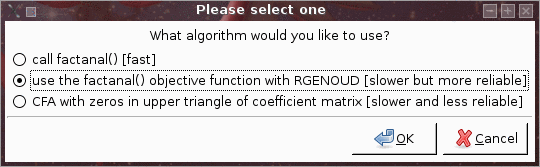
\includegraphics{screenshots/EFA/01}

The first option simply calls \Rcode{factanal()}, which is fine for
many problems and estimates the EFA model with the restrictions that
$\boldsymbol{\Lambda}^{\prime}\boldsymbol{\Theta}^{2}\boldsymbol{\Lambda}$
is diagonal and $\boldsymbol{\Phi}=\mathbf{I}$. The second algorithm
imposes these same restrictions but uses \Rcode{genoud()} to optimize
with a genetic algorithm. This approach is much slower but slightly
more likely to reach the global optimum in complicated problems The
third algorithm estimates the model under restrictions that $\boldsymbol{\Lambda}=\begin{bmatrix}\boldsymbol{\Lambda}_{1}\\
\boldsymbol{\Lambda}_{2}\end{bmatrix}$ where $\boldsymbol{\Lambda}_{1}$ is a $r_{1}\times r_{1}$ matrix
with zeros above the diagonal and $\boldsymbol{\Phi}=\mathbf{I}$. 

In principle, all three algorithms should produce the same estimate
of $\boldsymbol{\Theta}^{2}$ and be within a rotation of each other.
In practice, the third algorithm has difficulty meeting these standards.


\subsection{Factor Transformation}

Let $\boldsymbol{\Phi}=\mathbf{T}^{\prime}\mathbf{T}$ where $\mathbf{T}$
is a $r_{1}\times r_{1}$ transformation matrix with unit-length columns.
The factor transformation step chooses $\mathbf{T}$ so so that some
(lexical) objective function is \emph{minimized}. I initiated this
sequence with\\ \Rcode{mental.tests.rotated <- Rotate(mental.tests.efa)}


\subsubsection{Constraints}

Pe\~{n}a and Rodriguez (2003) defines a determinant of a correlation
matrix among a set of variables raised to the power of the reciprocal
of the number of variables as the ``effective variance'' of those
variables. The essence of the effective variance is that it can be
meaningfully compared to a different set of variables when the sets
of variables differ in size. The generalized variance is more well-known
statistic and is simply the determinant of the correlation matrix
among a set of variables. The generalized variance can be interpreted
as the hypervolume of a set of unit-length vectors and the effective
variance can be interpreted as {}``the length of the side of the
hypercube whose volume is equal to the determinant (Pe\~{n}a and
Rodriguez 2003, p.~363).'' Both of these concepts are used to define
the criteria / constraints in figure \ref{fig:constraints_EFA} to
be used while seeking the optimal $\mathbf{T}$.

%
\begin{figure}
\caption{Possible Constraints when Optimizing for $\mathbf{T}$ in EFA}
\label{fig:constraints_EFA}

\noindent \begin{centering}
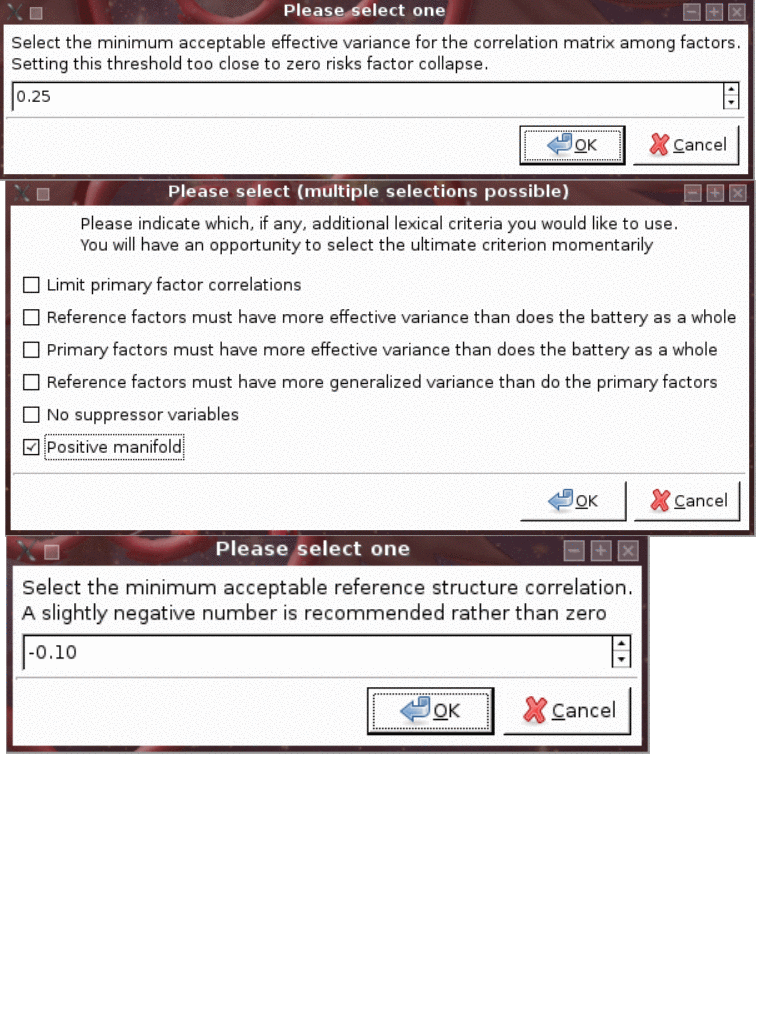
\includegraphics[scale=0.9]{screenshots/EFA/constraints}
\par\end{centering}
\end{figure}
The first criterion is required and prevents factor collapse. The
effective variance of the primary factors is defined as $\left|\boldsymbol{\Phi}\right|^{\frac{1}{r_{1}}}$.
If $\left|\boldsymbol{\Phi}\right|^{\frac{1}{r_{1}}}=0$, then $\boldsymbol{\Phi}$
and $\mathbf{T}$ are singular, a circumstance which is known as ``factor
collapse''. By specifying a non-zero threshold that the effective
variance must exceed, factor collapse can thus be prevented. In this
case, the threshold is $0.25$ and the criterion is formally defined
as\begin{eqnarray*}
 & \begin{cases}
-1 & \textrm{if}\,\left|\boldsymbol{\Phi}\right|^{\frac{1}{r_{1}}}\geq0.25\\
-\left(\left|\boldsymbol{\Phi}\right|^{\frac{1}{r_{1}}}\right) & \textrm{otherwise.}\end{cases}\end{eqnarray*}


The remaining constraints are optional and are enumerated in the next
dialog box in figure \ref{fig:constraints_EFA}. These criteria are
defined as follows:

\begin{itemize}
\item ``Limit primary factor correlations''. This option allows the user
to set valid intervals for pairwise corrleations between primary factors,
i.e. the off-diagonals of $\boldsymbol{\Phi}=\mathbf{T}^{\prime}\mathbf{T}$.
If this box is checked, dialog boxes that are similar to the previous
one will pop up asking for minimum and maximum acceptable correlations.
The associated criterion equals $-1$ if all off-diagonals are within
their valid intervals and equal to the distance between the most abberrant
correlation and the valid interval otherwise.
\item {}``Reference factors must have more effective variance than does
the battery as a whole''. This criterion is formally defined as\begin{eqnarray*}
 & \begin{cases}
1 & \textrm{if\,}\left|\boldsymbol{\Psi}\right|^{\frac{1}{r_{1}}}\leq\left|\mathbf{C}\right|^{\frac{1}{n}}\\
\left|\boldsymbol{\Psi}\right|^{\frac{1}{r_{1}}}-\left|\mathbf{C}\right|^{\frac{1}{n}} & \textrm{otherwise.}\end{cases}\end{eqnarray*}
This criterion loosely implies that the reference factors must be
{}``less correlated per variable'' than is the test configuration
in common factor space and encourages the first-order axes to cut
through the edges of the test configuration.
\item {}``Primary factors must have more effective variance than does the
battery as a whole''. This criterion is formally defined as\begin{eqnarray*}
 & \begin{cases}
1 & \textrm{if\,}\left|\boldsymbol{\Phi}\right|^{\frac{1}{r_{1}}}\leq\left|\mathbf{C}\right|^{\frac{1}{n}}\\
\left|\Phi\right|^{\frac{1}{r_{1}}}-\left|\mathbf{C}\right|^{\frac{1}{n}} & \textrm{otherwise,}\end{cases}\end{eqnarray*}
and is similar to the previous criterion above except that the correlation
among the primary factors at issue. In general, it seems that imposing
this restriction on the primary factors is \emph{stronger} than imposing
it on the reference factors and tends to push the first-order axes
farther out into the edges of the test configuration.
\item ``Primary factors must have less generalized variance than do reference
factors''. This criterion is extrapolated from Yates (1987, p.~27),
although it is not asserted with much formality in the text. Regardless,
the criterion could be operationalized as\begin{eqnarray*}
 & \begin{cases}
-1 & \textrm{if\,}\left|\boldsymbol{\Phi}\right|\leq\left|\boldsymbol{\Psi}\right|\\
\left|\boldsymbol{\Psi}\right|-\left|\boldsymbol{\Phi}\right| & \textrm{otherwise,}\end{cases}\end{eqnarray*}
but has a faster and substantively equivalent operationalization in
the code. When $r_{1}=2$, $\left|\boldsymbol{\Phi}\right|=\left|\boldsymbol{\Psi}\right|$
by necessity, so this criterion can bind only when $r_{1}\geq3$.
\item ``No suppressor variables''. Suppressor variables are defined as variables
with negative factor contributions. This criterion is advocated, albeit
somewhat indirectly, in Yates (1987, p.~119). Prohibiting suppressor
variables strikes me as a reasonable assumption to make in most cases.
The criterion is formally defined as \begin{eqnarray*}
-\frac{1}{nr}\sum_{j=1}^{n}\sum_{p=1}^{r}\mathbb{I}\left\{ \Gamma_{jp}\geq\underline{\Gamma}\right\}  & \textrm{where} & \mathbb{I}\left\{ \Gamma_{jp}\geq\underline{\Gamma}\right\} =\begin{cases}
1 & \textrm{if\,}\Gamma_{jp}\geq\underline{\Gamma}\\
0 & \textrm{otherwise,}\end{cases}\end{eqnarray*}
and $\underline{\Gamma}$ is a threshold for the minimum acceptable
factor contribution that is specified by the user. If this criterion
is checked, a pop-up will ask for the value of $\underline{\Gamma}$.
See the very end of section \ref{sub:maps} for a picture and explanation
of this dialog box, which is virtually identical to the next one.
\item ``Positive manifold''. This criterion is similar to (and a bit more
restrictive than) the criterion that prohibits suppressor variables.
The criterion is formally defined as\begin{eqnarray*}
-\frac{1}{nr}\sum_{j=1}^{n}\sum_{p=1}^{r}\mathbb{I}\left\{ \Upsilon_{jp}\geq\underline{\Upsilon}\right\}  & \textrm{where} & \mathbb{I}\left\{ \Upsilon_{jp}\geq\underline{\Upsilon}\right\} =\begin{cases}
1 & \textrm{if\,}\Upsilon_{jp}\geq\underline{\Upsilon}\\
0 & \textrm{otherwise,}\end{cases}\end{eqnarray*}
where $\underline{\Upsilon}$ is a threshold for the minimum acceptable
reference structure correlation that is specified by the user. If
this criterion is checked, the dialog box at the bottom of figure
\ref{fig:constraints_EFA}will ask for the value of $\underline{\Upsilon}$.
\end{itemize}

\subsubsection{The Ultimate Criterion}

%
\begin{figure}
\caption{Ultimate Criteria to be Used when Optimizing for $\mathbf{T}$ in
EFA}
\label{fig:ultimates}

\noindent \begin{centering}
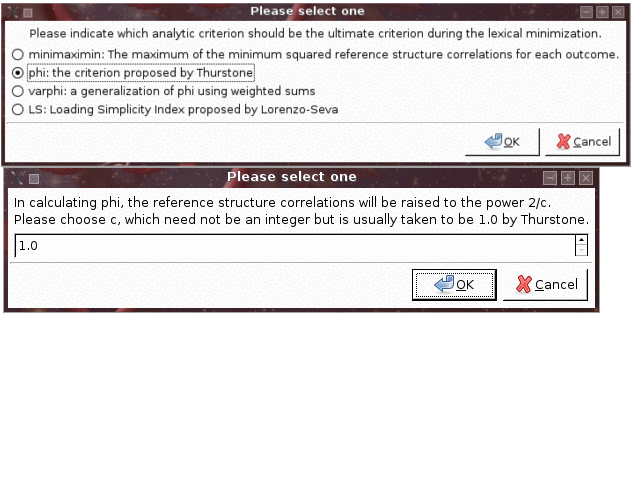
\includegraphics{screenshots/EFA/ultimates}
\par\end{centering}


\end{figure}
The final step is to choose the ultimate criterion for lexical optimization,
as shown in the dialog box in figure \ref{fig:ultimates}. These criteria
are defined as follows:

\begin{itemize}
\item minimaximin: This criterion attempts to satisfy Thurstone's definition
of simple structure by choosing $\mathbf{T}$ so that all outcomes
have at least one near-zero reference structure correlation. The criterion
is formally defined as \begin{eqnarray*}
 & \ln\left(\max\left\{ \min\left\{ \Upsilon_{1}^{2}\right\} ,\min\left\{ \Upsilon_{2}^{2}\right\} ,\dots,\min\left\{ \Upsilon_{n}^{2}\right\} \right\} \right).\end{eqnarray*}
Thus, the (log of the) maximum of the minimums of the squared rows
of $\boldsymbol{\Upsilon}$ is minimized. Taking the natural logarithm
just makes the optimization work a bit better near zero.
\item phi: This criterion was proposed by Thurstone (1935) to numerically
characterize simple structure when it reaches its theoretical minimum
of (log) zero. The criterion is formally defined as\begin{eqnarray*}
 & \ln\left(\sum_{j=1}^{n}\exp\left(\frac{1}{c}\sum_{p=1}^{r_{1}}\ln\left(\Upsilon_{jp}^{2}\right)\right)\right),\end{eqnarray*}
which is equal to logarithm of $\phi$ as defined by Thurstone (1935)
when $c=1$. Thurstone suggested that choosing $c$ to be greater
than $1.0$ could yield better results by lessening the pressure to
get one near-zero into each row of $\boldsymbol{\Upsilon}$ and increasing
the pressure to get more than one near-zero into some rows of $\boldsymbol{\Upsilon}$.
If Thurstone's criterion is used, the dialog box at the bottom of
figure \ref{fig:ultimates}will appear, prompting the user for $c$.
\item varphi: This criterion is a generalization of Thurstone's $\phi$.
Let $\overrightarrow{\boldsymbol{\Upsilon}}$ be a matrix of reference
structure correlations where each row is independently sorted in increasing
magnitude, and let $\underset{-\left[1:p\right]}{\overrightarrow{\phi}}$
be Thurstone's criterion (with $c=1$) calculated on $\overrightarrow{\boldsymbol{\Upsilon}}$,
excluding the first through the $p$th column of $\overrightarrow{\boldsymbol{\Upsilon}}$.
Then define $\varphi=\phi+\sum_{p=1}^{r-2}w_{p}\underset{-\left[1:p\right]}{\overrightarrow{\phi}}$,
where $w_{p}\in\left[0,1\right]$ is the weight the analyst specifies
for $\underset{-\left[1:p\right]}{\overrightarrow{\phi}}$ relative
to a unit weight placed on $\phi$. At one extreme, if $w_{p}=0\,\forall p$,
then $\varphi=\phi$. At the other extreme, if $w_{p}=1\,\forall p$,
then the analyst favors a perfect cluster configuration, where three
is only one non-zero coefficient per test. An ``objective'' alternative
to specifying weights is to specify that the weights are a function
of $\overrightarrow{\boldsymbol{\Upsilon}}$, such as $w_{p}=\max\left\{ 0,1-\max\left\{ \overrightarrow{\Upsilon}_{\left(p+1\right)}^{2}\right\} \right\} $
to gradually reduce the weight as $p$ increases. If this criterion
is chosen, the dialog boxes in figure \ref{fig:weights} will appear,
prompting the user to specify whether dynamic weights or static weights
should be used. If user-specified weights are chosen, the user is
then prompted to specify each $w_{p}$ .
\item LS: This criterion is called the Loading Simplicy Index in Lorenzo-Seva
(2003). The derivation of it is not complicated but involves a lot
of notation not previously introduced here, so the reader is refered
to Lorenzo-Seva (2003) for details. Simply put, it reaches its optimum
of (negative) $1.0$ when $\boldsymbol{\Upsilon}$ exhibits a perfect
cluster configuration. Although Lorenzo-Seva (2003) defines the Loading
Simplicity Index in terms of the primary pattern matrix, it is invariant
to the column-scale of the primary pattern matrix and thus can arbitrarily
be defined for the reference structure matrix as well.%
\begin{figure}
\caption{Weights for the $\varphi$ Criterion}
\label{fig:weights}

\noindent \begin{centering}
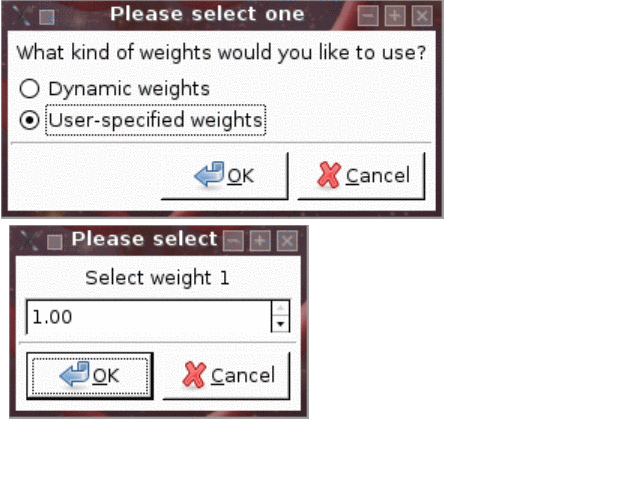
\includegraphics{screenshots/EFA/varphi}
\par\end{centering}


\end{figure}

\end{itemize}

\section{References}

{\small Butler, J.M. 1969. ``Simple Structure Reconsidered: Distinguishability
and Invariance in Factor Analysis.'' }\emph{\small Multivariate Behavioral
Research}{\small{} 4(1):5\textendash{}28.}{\small \par}

{\small Goodrich, B. 2008a. ``SEFA$i$R So Far.'' Unpublished manuscript
available from the FAiR wiki \url{http://wiki.r-project.org/rwiki/doku.php?id=packages:cran:fair}}{\small \par}

{\small Goodrich, B. 2008b. ``Analytic Transformation of Factors in
FA$i$R.'' Unwritten manuscript. Email me about it.}{\small \par}

{\small Howe, W.G. 1955. Some Contributions to Factor Analysis. Technical
report ORNL-1919, Oak Ridge National Lab., Tenn.}{\small \par}

{\small Lorenzo-Seva, U. 2003. \textquotedblleft{}A factor simplicity
index.\textquotedblright{} }\emph{\small Psychometrika}{\small{} 68(1):49\textendash{}60.}{\small \par}

{\small Pe\~{n}a, D. and J. Rodriguez. 2003. ``Descriptive measures
of multivariate scatter and linear dependence.'' }\emph{\small Journal
of Multivariate Analysis}{\small{} 85(2):361\textendash{}374.}{\small \par}

{\small Thurstone, L.L. 1935. }\emph{\small The vectors of mind: multiple-factor
analysis for the isolation of primary traits}{\small . University
of Chicago Press.}{\small \par}

{\small Yates, A. 1987. }\emph{\small Multivariate exploratory data
analysis: A perspective on exploratory factor analysis}{\small . State
University of New York Press.}
\end{document}
